\documentclass[oneside, 11pt]{article}

\usepackage[T1]{fontenc}
\usepackage[utf8]{inputenc}
\usepackage[english]{babel}
\usepackage{enumerate}
\usepackage{isotope}


\usepackage{fouriernc}
\usepackage[detect-all, binary-units, separate-uncertainty=true,
            per-mode=symbol, retain-explicit-plus, retain-unity-mantissa=false]{siunitx}

\usepackage{setspace}
\setstretch{1.2}

\setlength{\parskip}{\smallskipamount}
\setlength{\parindent}{0pt}

\usepackage[headheight=14pt]{geometry}
\geometry{marginparwidth=0.5cm, verbose, a4paper, tmargin=3cm, bmargin=3cm,
          lmargin=2cm, rmargin=2cm}

\usepackage{float}

\usepackage[fleqn]{amsmath}
\numberwithin{equation}{section}
\numberwithin{figure}{section}

\usepackage{graphicx}
\graphicspath{{images/}{../../../images/}}

\usepackage{tikz}
\usetikzlibrary{shapes}
\usetikzlibrary{plotmarks}

\newcounter{Exercise}
\setcounter{Exercise}{1}
\usepackage{xcolor}
\definecolor{shadecolor}{gray}{0.9}
\usepackage{framed}
\usepackage{caption}

\usepackage{url}


\usepackage{fancyhdr}
\pagestyle{fancy}
\fancyhf{}
\rhead{\thepage}
\renewcommand{\footrulewidth}{0pt}
\renewcommand{\headrulewidth}{0pt}

\fancypagestyle{firststyle}
{
    \fancyhf{}
    \rhead{\thepage}
    \cfoot{\includegraphics[height=30pt]{HiSPARClogo}}
    \rfoot{\includegraphics[height=25pt]{CCbysa}}
    \lfoot{
\includegraphics[height=30pt]{NIKHEFlogo}}
    \renewcommand{\footskip}{50pt}
    \renewcommand{\footrulewidth}{0.1pt}
    \renewcommand{\headrulewidth}{0pt}
}

\newcommand{\figref}[1]{Figuur~\ref{#1}}

\newcommand{\hisparc}{\textsmaller{HiSPARC}\xspace}
\newcommand{\kascade}{\textsmaller{KASCADE}\xspace}
\newcommand{\sapphire}{\textsmaller{SAPPHiRE}\xspace}
\newcommand{\jsparc}{\textsmaller{jSparc}\xspace}
\newcommand{\hdf}{\textsmaller{HDF5}\xspace}
\newcommand{\aires}{\textsmaller{AIRES}\xspace}
\newcommand{\csv}{\textsmaller{CSV}\xspace}
\newcommand{\python}{\textsmaller{PYTHON}\xspace}
\newcommand{\corsika}{\textsmaller{CORSIKA}\xspace}
\newcommand{\labview}{\textsmaller{LabVIEW}\xspace}
\newcommand{\daq}{\textsmaller{DAQ}\xspace}
\newcommand{\adc}{\textsmaller{ADC}\xspace}
\newcommand{\hi}{\textsc{h i}\xspace}
\newcommand{\hii}{\textsc{h ii}\xspace}
\newcommand{\mip}{\textsmaller{MIP}\xspace}
\newcommand{\hisparcii}{\textsmaller{HiSPARC II}\xspace}
\newcommand{\hisparciii}{\textsmaller{HiSPARC III}\xspace}

\DeclareSIUnit{\electronvolt}{\ensuremath{\mathrm{e\!\!\:V}}}

\DeclareSIUnit{\unitsigma}{\ensuremath{\sigma}}
\DeclareSIUnit{\mip}{\textsmaller{MIP}}
\DeclareSIUnit{\adc}{\textsmaller{ADC}}

\DeclareSIUnit{\gauss}{G}
\DeclareSIUnit{\parsec}{pc}
\DeclareSIUnit{\year}{yr}




%document details
\author{N.G. Schultheiss \\ translated and adapted by K. Schadenberg}
\date{}
\title{The Expanding Universe}


\begin{document}
\maketitle

\section{Introduction}
This module `The Expanding Universe' follows the modules `The Universe' and `Telescopes'. This module tries to explain the discovery of the expanding universe. From the idea that the universe is expanding also follows the notion that it used to be smaller. Long ago the entire universe was infinitely small. From this the theory of the `Big Bang' originates.

\section{Vesto Slipher}
Vesto Melvin Slipher, an American astronomer, used spectrographic techniques\footnote{With spectrographic research one looks at the spectrum of light, the colours, emitted by an object.} to determine the rotation and orbital period\footnote{As with most terms in astronomy, we need to be very careful about the meaning of words. One rotation period is the time it takes an object to complete one revolution around its axis of rotation. This is measured against the background starts. This means that for our planet, the Earth, one day is not the same as one rotation period. One (solar) day is measured with respect to the Sun and is therefore longer than the rotation period because it includes a part of the orbital period. One orbital period is the time it takes one celestial body, in this case the Earth, to complete one orbit around another celestial body, in this case the Sun.} of planets. Some planets are surrounded by cloud cover. As a consequence we cannot see the surface of the planets and details are blurred. We can however try to measure the velocity of the gas (the atmosphere) on both sides of the planes, one side will come towards us, the other will move away from us. Using this we can estimate the rotation period of the planet.

Measuring the speed of moving gasses millions of kilometres away is not straightforward. We can however use a small trick. As explained in the modules `The Sun' and `Colour', every atom has his own colour signature, a specific spectrum of absorption/emission lines. You may have heard about the Doppler effect. A police car with its sirens on sounds different when it is driving towards you (higher pitch) then when it is driving away from you (lower pitch). The same Doppler shift also happens with light. When an object moves towards you with high speed, the light you perceive from this object seems bluer. If we can measure the colour shift of the absorption lines we can use the equation for the Doppler effect to calculate the speed of the object. If the speed of a planet is known one can calculate its orbital period.

\begin{shaded}
\textbf{Exercise \theExercise \stepcounter{Exercise}} : If an object moves away from you with great speed, to what colour is the light coming from the object shifted? Explain your answer using the terms wavelength and frequency.\end{shaded}

\begin{figure}\begin{center}
\begin{picture}(0,0)%
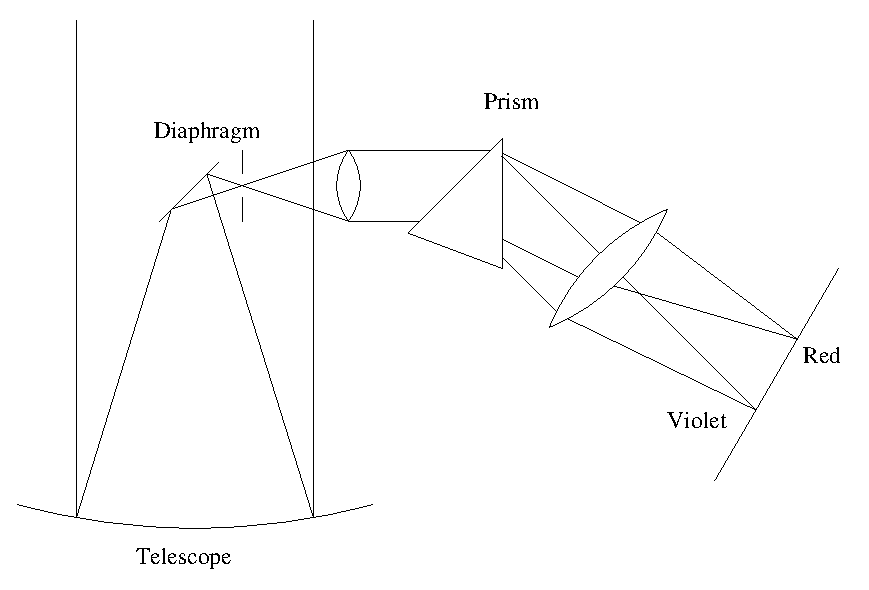
\includegraphics{spectroscope}%
\end{picture}%
\setlength{\unitlength}{4144sp}%
%
\begingroup\makeatletter\ifx\SetFigFont\undefined%
\gdef\SetFigFont#1#2#3#4#5{%
  \reset@font\fontsize{#1}{#2pt}%
  \fontfamily{#3}\fontseries{#4}\fontshape{#5}%
  \selectfont}%
\fi\endgroup%
\begin{picture}(6361,4225)(443,-3734)
\end{picture}%
\caption{Schematic representation of a telescope equipped with a spectroscope.}\label{fig:spectroscope}
\end{center}\end{figure}

Figure~\ref{fig:spectroscope} is a schematic representation of a setup which can be used to measure colour shifts. The atoms in the atmosphere of a planet absorb certain types of light. These become dark lines in the spectrum of light coming from the planet. The spectrum is made by refracting the light using a prism. Every colour is refracted over a different angle, this creates the spectrum. If all the light from the planet is passed through the prism, the different colours would overlap. By using a diaphragm we can block a part of the light. This enables us to look at only a small region of a planet and prevents the blurring of colours. In figure~\ref{fig:spectroscope} the diaphragm is placed directly after the second mirror in the telescope, this is a relatively simple design. More complicated designs use an extra lens before the prism and place the diaphragm just before the prism, this results in more clear spectra.

\section{Doppler effect}
All waves, including light waves, can be completely described using two of the following three quantities:
\begin{description}
\item[Wavelength $\lambda$]; the length of the wave, measured in metres [m].
\item[Frequency $f$]; the number of vibrations per second, measured in Hertz [Hz] or number per second [s$^{-1}$]. In sound this determines the pitch or the tone of the sound, in light the colour. Instead of frequency one could also use the period (of oscillation) $T$ (the duration of one cycle), which is equal to $T=\frac{1}{f}$.
\item[Wave propagation speed $v$];  the speed at which the waves are propagating through the medium. For light in vacuum this is the speed of light\footnote{Remember that `the speed of light' can mean the speed of light in vacuum (as used here), or the speed of light in a specific other medium.}, $c=299792458~\mbox{m s}^{-1}$, measured in metres per second [m/s or m s$^{-1}$]
\end{description}
These three quantities are linked to each other as described in the following equation:
\begin{equation} v = \lambda f \label{eq:wave}
\end{equation}

A forth quantity associated with waves is the phase $\phi$. This quantity has two closely related but different meanings. One is the initial angle of the wave (when described as a sinusoidal function) at its origin, sometimes this is called the phase offset to distinguish it from the second meaning. The second meaning of the word phase is the fraction of the wave cycle which has passed relative to the origin. This is the wrapped phase because it is constrained to an interval such as $\left( -\pi , pi\right]$, $\left[ 0,2\pi\right)$ or a percentage/fraction. The unwrapped phase is the total number of wave cycles (or parts thereof) which have passed.

\subsection{Doppler and sound waves}
We start by looking at Doppler effects at low speeds. In doing this we can, for now, ignore relativistic effects.\footnote{See the module `Relativity' for more information about relativistic effects. For now we will simple state that when you go really fast, time and space seem to change.} We will use sound waves in the following equations, with a speed $v_{\mbox{\begin{tiny}sound\end{tiny}}}$. We will be looking at a single source - observer pair, one will be stationary and the other will move at a speed slower than the speed of sound. The speed of the sound source will be denoted as $v_{\mbox{\begin{tiny}source\end{tiny}}}$, of the observer as $v_{\mbox{\begin{tiny}observer\end{tiny}}}$. 

In figure~\ref{fig:doppler_1} we see the location of (sound) wave crests and troughs emitted by a moving source. From this figure the influence of movement on the wavelength can be clearly seen.
\begin{figure}[t]\begin{center}
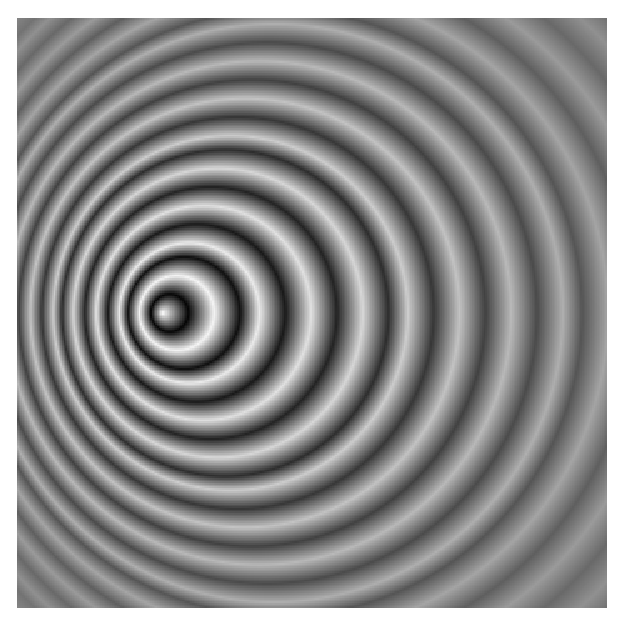
\includegraphics[scale=1]{Doppler_effect.svg.eps}%
\caption{The Doppler effect. The source of the waves in this figure is moving to the left. Notice that the distance between the wave crests is different on the left and right side of the source.}\label{fig:doppler_1}
\end{center}\end{figure}

\begin{shaded}
\textbf{Exercise \theExercise \stepcounter{Exercise}} : Explain in your own words the effect of a moving sound source on the pitch of the observed sound (i.e. How does an ambulance siren sound when it is approaching you and how does it sound when it is moving away?) Use the term wave length in your explanation and refer to figure~\ref{fig:doppler_1}.\end{shaded}

For the Doppler effect it is important which object is moving and in what direction. With this in mind we will take a slightly different look at the Doppler effect. In figure~\ref{fig:doppler_1d} we see the sound wave emitted by a source located in the origin of the graph. The start of the first wave has propagated a certain distance determined by the speed of sound:
\begin{equation*}
s_{\mbox{\begin{tiny}sound\end{tiny}}}=v_{\mbox{\begin{tiny}sound\end{tiny}}} t
\end{equation*}
In the same figure the location of an observer is indicated with an arrow. This observer was not stationary but moved along with the sound waves at a constant speed, also starting at the origin. It location is given by:
\begin{equation*}
s_{\mbox{\begin{tiny}observer\end{tiny}}}=v_{\mbox{\begin{tiny}observer\end{tiny}}} t
\end{equation*}
What was the effect on the sound as heard by the observer? The source has emitted three complete periods of the sound, but the observer has only heard slightly move than two go past:
\begin{equation*}
\phi_{\mbox{\begin{tiny}observer\end{tiny}}} = \frac{v_{\mbox{\begin{tiny}sound\end{tiny}}} - v_{\mbox{\begin{tiny}observer\end{tiny}}}}{v_{\mbox{\begin{tiny}sound\end{tiny}}}} \phi_{\mbox{\begin{tiny}source\end{tiny}}}
\end{equation*}

\begin{figure}\begin{center}
\begin{picture}(0,0)%
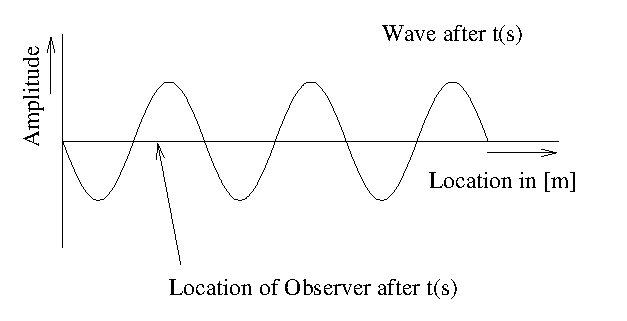
\includegraphics{doppler_1}%
\end{picture}%
\setlength{\unitlength}{4144sp}%
%
\begingroup\makeatletter\ifx\SetFigFont\undefined%
\gdef\SetFigFont#1#2#3#4#5{%
  \reset@font\fontsize{#1}{#2pt}%
  \fontfamily{#3}\fontseries{#4}\fontshape{#5}%
  \selectfont}%
\fi\endgroup%
\begin{picture}(4510,2179)(459,-1394)
\end{picture}%
\caption{Wave emitted by a source at the origin with a moving observer.}\label{fig:doppler_1d}
\end{center}\end{figure}

Because of the velocity of the observer with respect to the source, the crests of the waves arrived less frequently at the observer:
\begin{equation}
f_{\mbox{\begin{tiny}observer\end{tiny}}} = \frac{v_{\mbox{\begin{tiny}sound\end{tiny}}} - v_{\mbox{\begin{tiny}observer\end{tiny}}}}{v_{\mbox{\begin{tiny}sound\end{tiny}}}} f_{\mbox{\begin{tiny}source\end{tiny}}} \label{eq:doppler_f_obs}
\end{equation}
The change in frequency, or Doppler shift is then equal to:
\begin{align}
\Delta f &= f_{\mbox{\begin{tiny}observer\end{tiny}}} - f_{\mbox{\begin{tiny}source\end{tiny}}}= \frac{v_{\mbox{\begin{tiny}sound\end{tiny}}} - v_{\mbox{\begin{tiny}observer\end{tiny}}}}{v_{\mbox{\begin{tiny}sound\end{tiny}}}} f_{\mbox{\begin{tiny}source\end{tiny}}} - f_{\mbox{\begin{tiny}source\end{tiny}}} \\
\Delta f &= \left( \frac{v_{\mbox{\begin{tiny}sound\end{tiny}}} - v_{\mbox{\begin{tiny}observer\end{tiny}}}}{v_{\mbox{\begin{tiny}sound\end{tiny}}}} -1 \right)  f_{\mbox{\begin{tiny}source\end{tiny}}}
 \label{eq:f_delta_away}
\end{align}

\begin{shaded}
\textbf{Exercise \theExercise \stepcounter{Exercise}} : How do the equations above change when the source is moving instead of the observer?

Extra: Can you write down a equation which is valid for all cases (source and/or observer are moving in either direction)? \end{shaded}

\subsection{Doppler effect and light}
Equations~\ref{eq:doppler_f_obs} and \ref{eq:f_delta_away} of the previous section are nearly identical for light. If the observer and source are moving at speeds far below the speed of light and straight towards or away from each other the following equations are valid:
\begin{align}
f &= \left(1 - \frac{v_{\mbox{\begin{tiny}source,observer\end{tiny}}}}{c}\right) f_0 \\
\Delta f &= - \frac{v_{\mbox{\begin{tiny}source,observer\end{tiny}}}}{c} f_0 \label{eq:dopp_light} 
\end{align}
$v_{\mbox{\begin{tiny}source,observer\end{tiny}}}$ is the velocity of the source relative to the observer, this number is positive when the two are moving away from each other.

When the speed of either the observer of source approaches the speed of light equation~\ref{eq:dopp_light} is no longer valid. The derivation of the correct equations compensating for relativistic effects is beyond the scope of this text. Here we will only give the correct formula to use. When you completed the module `Relativity' you might want to come back to this module to see if you can derive the equations below.
\begin{equation}
f = \sqrt{\frac{1-\frac{v}{c}}{1+\frac{v}{c}}} f_0 \label{eq:dopp_light_rel} 
\end{equation}
It is common practice to shorten the ratio $\frac{v}{c}$ to $\beta$. The equation for the frequency shift then becomes:
\begin{equation}
\Delta f = \left( 1-\sqrt{\frac{1-\beta}{1+\beta}} ~\right)  f_0  \label{eq:dopp_shift_light_rel} 
\end{equation}
The ratio:
\begin{equation}
\frac{f}{f_0}= \sqrt{\frac{1+\beta}{1-\beta}} \label{eq:dopp_factor} 
\end{equation}
is called the Doppler factor (source relative to observer), this term is often used in astrophysics.

\begin{shaded}
\textbf{Exercise \theExercise \stepcounter{Exercise}} : Vesto Slipher discovered that the Andromeda nebula is coming towards us with a speed of 300 kilometres per second. Was it necessary to use equation~\ref{eq:dopp_shift_light_rel} or was equation~\ref{eq:dopp_light} still valid at this speed?\\
Hint: How large is the difference in the calculated colour shift between the equations at this speed?
\end{shaded}

\section{Hubble and Lema\^itre}
Edwin Powell Hubble had access to a 100" telescope, at that time the largest telescope on Earth. Because of its large size the telescope had an excellent resolution which allowed Hubble to distinguish real nebulas from galaxies which appeared to be nebulas because of the large distances. During his many observations he noticed that almost all galaxies move away from the Milky Way and not towards it like Andromeda.

Furthermore, is seemed as though galaxies further away had higher speeds, all away from us. Hubble determined the velocity of a large number of galaxies and found a relationship between the distance and speed. This is now known as Hubble's law and the value of the rate of expansion is called the Hubble constant. Although the law is called after Hubble, it was first derived from General Relativity by Georges Henri Joseph \'Edouard Lema\^itre.

Lema\^itre came to the conclusion that, if his hypothesis was right, the universe must have had a beginning, when all the mass was close to each other, or even at one point in space. Lema\^itre's own description was that the Cosmic Egg exploded at the moment of creation. By other scientist this bizarre idea became ridiculed, but later widely accepted as the Big Bang theory.

The Hubble constant is roughly 75~km/sMpc, kilometres per second per Megaparsec. One Parsec is a little over 3.25~light~year. We could therefore also say that the Hubble constant is 23~km~s$^-1$ per megalight year. An object 10 Megaparsec away will move away from us at a speed of 230 kilometres per second.

\begin{shaded}
\textbf{Exercise \theExercise \stepcounter{Exercise}} : The age of the universe has been determined to be somewhere in the neighbourhood of 13.6 billion years. This means that light emitted at the beginning of the universe could have, at most, travelled 13,6 billion light years. If this is the edge of the universe, how fast is it moving away from us? Does this answer surprise you?\end{shaded}

\section{Research into the Big Bang}
If the universe started with the Big Bang then we must be able to prove this with the help of experiments.\footnote{Proving can be a difficult concept in the sciences. With the scientific method we can make predictions about how the world around us should work if a certain hypotheses is correct. With experiments we then test if our predictions are correct. If the results of the experiments contradict our predictions we have proved that our hypothesis is wrong. If however the results agree with the predictions we have evidence supporting our hypothesis. This means it might be correct, but only until it is proven wrong.

As an example Newton's Laws were `proven' to be right. But only until we discovered small differences between actual orbit of Mercury around the Sun and its predicted orbit according to these laws. This took several hundred years and in the meantime the theory was temporarily correct.

In short we can disprove any definite theory wrong, but never right.} Because of the Doppler shifts involved we must look at very long wave lengths; infra red waves or even radio waves. Measuring these waves was done in 1983 by the IRAS-satellite. 

\begin{shaded}
\textbf{Exercise \theExercise \stepcounter{Exercise}} : Why were the infra red and radio waves measured in space and not on Earth?\end{shaded}
\begin{shaded}
\textbf{Exercise \theExercise \stepcounter{Exercise}} : Why does an infra red telescope have a larger mirror than a telescope used for visible light?\end{shaded}
\begin{shaded}
\textbf{Exercise \theExercise \stepcounter{Exercise}} : What is the resolution of the Hubble-telescope (for visible light) and the IRAS-telescope (for infra red light). How large is the difference?\end{shaded}

\end{document}